\documentclass[11pt]{amsart}
\usepackage{graphicx}
\usepackage{amsaddr}
\usepackage{hyperref}
\usepackage{amsmath,amssymb}

\textwidth=6in
\textheight=9.5in
\headheight.2cm
\topmargin-0.5in
\evensidemargin0.25in
\oddsidemargin0.25in
\def\baselinestretch{1.25}\large\normalsize

\hbadness3000
\vbadness30000
\parindent=0.3in
\parskip=3pt plus 1pt minus 1pt

% ------------------------------------------------------------------------------------------------------
\usepackage[most]{tcolorbox}
\usepackage{caption, xcolor}

\usepackage{tikz, pgfplots}
\usepgflibrary{shadings}
\usetikzlibrary{positioning, shapes.geometric, fit, arrows.meta}
\pgfplotsset{compat=1.18}

%-------------------------------------------------------------------------------------------------
\theoremstyle{plain}
\newtheorem{theorem}{Theorem}[section]
\newtheorem{lemma}[theorem]{Lemma}
\newtheorem{corollary}[theorem]{Corollary}
\newtheorem{algorithm}[theorem]{Algorithm}

\theoremstyle{definition}
\newtheorem{definition}[theorem]{Definition}
\newtheorem{example}[theorem]{Example}
\newtheorem{remark}[theorem]{Remark}

\numberwithin{equation}{section}
\setcounter{page}{25}

\begin{document}
	\newcommand{\T}{\mathbb{T}}
	\newcommand{\R}{\mathbb{R}}
	\newcommand{\Q}{\mathbb{Q}}
	\newcommand{\N}{\mathbb{N}}
	\newcommand{\Z}{\mathbb{Z}}
	\newcommand{\tx}[1]{\quad\mbox{#1}\quad}
	%Please put here any further newcommands.
	%\hfill  123\\
	\noindent {\tt The Nepali Math. Sc. Report\\
		Vol. 41, No.1 and 2, 2024\\}


\title [Applications of Galois Theory]
{Applications of Galois Theory}
\author[Sandesh Thakuri, Bishnu Hari Subedi]{Sandesh Thakuri$^1$ \and Bishnu Hari Subedi$^2$}
\address{
  $^{1,2}$ Central Department of Mathematics, TU, Nepal\\[-2mm]
  {\tiny sandeshthakuri111@gmail.com}}

\vspace{-.2cm}
\thanks{\hspace{-.5cm}\tt
	Received  May 1, 2024
	\hfill }


\maketitle
\thispagestyle{empty}

{\footnotesize
  \noindent{\bfseries Abstract:} {This paper gives an insight to the Galois Theory and discusses its applications in both pure and applied mathematics. First the fundamental theorem of Galois Theory is introduced which is then applied to compute the Galois groups of polynomials and to prove the non existence of formula for solving a polynomial equations in rationals having degree greater than four. Then the finite fields called the Galois fields are introduced with their applications in error correcting codes and cryptography in computer science. There are no general rules to compute the Galois groups of polynomials of degree more than four. Two new examples of Galois groups of polynomials of degree greater than four are also introduced and the concept of Galois group of a  single variable polynomial is extended to the Galois group of a multi-variable polynomial.}\\

  \noindent{\bfseries Key Words}: Fundamental Theorem, Galois Group, Galois Field, Error correcting codes, Cryptography\\
  \bfseries AMS (MOS) Subject Classification.} 12F10, 11R32

\vspace{4mm}
 \section{Introduction}
 The foundation of Galois Theory was laid by the French Mathematician \textit{Évariste Galois}(1811-1832) by determining the necessary and sufficient condition for solving a polynomial equation by radicals and thereby solving the problem that was open for 350 years old \cite{galois}. Modern Galois Theory is a theory of field extension which is a vast theory. The core-part of the Galois Theory is the ``Fundamental Theorem of Galois Theory'' \cite {hunger}  which links two main parts of Abstract Algebra; Field Theory and Group Theory. This is a profound result in Abstract Algebra.\\

 \subsection{The Fundamental Theorem}
 Let \(F\) be an extension field of a field \(K\).

 \begin{definition} \cite{hunger} [Galois Group]
  The group of all K-automorphisms of \(F\) is called the Galois group of \(F\) over \(K\) and it is denoted by \(Aut_K^F\).
\end{definition}

\begin{definition} \cite{hunger} [Galois Extension]
Let \(F\) be an extension field of \(K\) such that the fixed field of the Galois group \(Aut_k^F\) is \(K\) itself. Then \(F\) is said to be a Galois extension of \(K\) or Galois over K.
\end{definition}

\begin{theorem} \cite{hunger} [The Fundamental Theorem]
  If \(F\) is a finite dimensional Galois extension of \(K\), then there is a one-to-one correspondence between the set of all intermediate fields of \(F\) over \(K\) and the set of subgroups of the Galois group \(Aut_K^F\) such that:
  \begin{enumerate}
  \item[i)] the relative dimension of two intermediate fields is equal to the relative index of the corresponding subgroups. In particular \(Aut_K^F\) has order \([F:K]\);
  \item[ii)] \(F\) is Galois over every intermediate field \(E\), but \(E\) is Galois over \(K\) if and only if the corresponding subgroup \(E'= Aut_E^F\) is normal in \(G=Aut_K^F\).In this case \(G/E'\) is isomorphic to the Galois group \(Aut_K^E\) of \(E\) over \(K\).
  \end{enumerate}
\end{theorem}

The fundamental theorem links Field theory to Group theory. This allows us to use the tools of Group theory to solve the problems involving field theory. Solving a polynomial equation is a problem of field theory. We can use insights of Group theory to solve this problem of field theory which is discussed in some detail.

\subsubsection{Insights to the Fundamental Theorem}

\textbf{Nature of a Number}\\
The nature of a number depends upon the underlying field. \(\sigma:\{a+b\sqrt{2}\} \mapsto \{a-b\sqrt{2}\}\) where \(a,b \in \mathbb{Q}\) is a field-automorphism of  \(\mathbb{Q}(\sqrt{2})\) that fixes \(\mathbb{Q}\). This map \(\sigma \) is also denoted by \(\sqrt{2} \longmapsto -\sqrt{2}\). So, any polynomial equation over \(\mathbb{Q}\) satisfied by the number \(\sqrt{2}\) is also satisfied by the number \(-\sqrt{2}\). You can fluidly pass between these two numbers and the equation with a rational coefficient will not know. Hence the two numbers \(\sqrt{2}\) and \(-\sqrt{2}\) are algebraically same over \(\mathbb{Q}\).\\

But the map \(\sqrt{2} \longmapsto -\sqrt{2}\) does not fix the field \(\mathbb{Q}(\sqrt{2})\) i.e does not fix itself. The only automorphism of \(\mathbb{Q}(\sqrt{2})\) is the identity map. So, you cannot pass \(\sqrt{2}\) for \(-\sqrt{2}\) for every equation with coefficients in \(\mathbb{Q}(\sqrt{2})\). Hence the two numbers \(\sqrt{2}\) and \(-\sqrt{2}\) are not algebraically same over \(\mathbb{Q}(\sqrt{2})\).

\begin{figure}[h]
  \centering
  \small
 \begin{tikzpicture}
      \node (f) {\(\mathbb{Q}(\sqrt{2})\)};
      \node[below of=f, yshift=-17mm] (e) {\(\mathbb{Q}\)};


      \draw[<-,thick] (f)--(e);

      \node[right of=f, xshift=55mm] (i) {\{e\}};
      \node[below of=i, yshift=-17mm] (h) {\{\(i\), \(\sqrt{2} \mapsto -\sqrt{2}\)\}};


      \draw[->, thick] (i)--(h);


      \draw[<->, thick] (f)--(i);
      \draw[<->, thick] (e)--(h);
    \end{tikzpicture}
    \caption{\footnotesize Field containing \(\sqrt{2}\)}
    \end{figure}

\textbf{Structure of a Field}\\
The structure of a field as an extension field over some field is mirrored in the structure of the ``group'' of  permutations of its elements that keeps the base field fixed. But these permutations are the symmetries of the field. \textit{So, the structure of field extension is equals to its own symmetry.}\\

The structure of a field is a complicated thing; specially if it is infinite. But the structure of a group is rather simple; especially if it is finite. So the Galois theory has fairly simplified the complicated thing in a very insightful and beautiful way.\\

Also Galois theory gives a new sights of study of fields which is ``study of fields via study of its automorphisms'' which are permutations of the field. That is,

\begin{figure}[h]
  \begin{tikzpicture}

    \node[rectangle, thick, draw,
    minimum height=3.7cm,
    minimum width=2.5cm] (rec) at (0,0) {};

    \node[rectangle, thick, draw,
    minimum height=3.7cm,
    minimum width=2.5cm] (rec2) at (6,0) {};


    \node[minimum width=7mm,
      minimum height=7mm,
      fill=gray!40,
      ] (ss) at (0,2.3) {Structure of a field \(F\)};

      \node[minimum width=7mm,
      minimum height=7mm,
      fill=gray!40,
      ] (ss2) at (6,2.3) {Structure of its symmetry};

      \draw[<->, thick] (ss)--(ss2);
      \draw[<->, thick] (rec)--(rec2);

      \node[minimum width=7mm,
      minimum height=7mm,
      fill=gray!40] (f) at (0,1.2) {F};

      \node[minimum width=7mm,
      minimum height=7mm,
      fill=gray!40,
      below of=f, yshift=-3mm] (e) {E};

      \node[right of=e,
      xshift=20mm, yshift=3mm] (txt) {Equivalent};


      \node[minimum width=7mm,
      minimum height=7mm,
      fill=gray!40,
      below of=e, yshift=-3mm] (k) {K};

      \draw[<-,thick] (f)--(e);
      \draw[<-,thick] (e)--(k);

      \node[right of=f,
      xshift=5cm,
      minimum width=7mm,
      minimum height=7mm,
      fill=gray!40,
      ] (i) {\{e\}};

      \node[minimum width=7mm,
      minimum height=7mm,
      fill=gray!40,
      below of=i, yshift=-3mm] (h) { H};

      \node[
      minimum width=7mm,
      minimum height=7mm,
      fill=gray!40,
      below of=h, yshift=-3mm] (g) {G};

      \draw[->, thick] (i)--(h);
      \draw[->, thick] (h)--(g);
    \end{tikzpicture}
    \caption{\footnotesize Equivalency}
  \end{figure}

\subsection{Galois Field}
 Fields having only finite number of elements are called Galois field. We denote Galois field with \(q\) elements by \(GF(q)\). Basically there are two types of representation of a finite field. These two representations are equivalent.\\

\textbf{Integer representation}\\
\(GF(p^n)=\{0,1,...,p-1\} \cup \{p,p+1,...,p+p-1\} \cup ... \cup \{p^{n-1},p^{n-1}+1,...,p^{n-1}+p^{n-2}+...+p-1\}\) \cite{galois}.

\begin{example}
    \(GF(2)=\{0,1\}\)\\
    \(GF(2^3)=\{0,1\} \cup \{2,2+1\} \cup \{2^2,2^2+1,2^2+2,2^2+2+1\}=\{0,1,2,3,4,5,6,7\}\)
\end{example}

But the digits \(2,3,..,7\) of the field \(GF(2^3)\) do not lie on the field \(GF(2)\). If we look the field \(GF(2^3)\) as an extension field of \(GF(2)\) and write its elements using only the elements of the base field \(GF(2)\) then we have the following representations:

\begin{table}[h!]
  \centering
\begin{tabular}{|c|c|c|}
    \hline
    Digits & Expansion & Binary rep..\\
    \hline
    3 & \(2+1\) & 011 \\
    4 & \(2^2+2^1 \times 0 +2^0 \times 0\) & 100 \\
    5 & \(2^2+1\) & 110 \\
    \hline
\end{tabular}
\caption{\small Binary representation table of field elements.}
\end{table}

This is actually Binary representation of the field \(GF(2^3)\).\\

\textbf{Polynomial representation}\\
For a field \(F\) and an irreducible polynomial \(f(x) \in F[x]\) the quotient ring \(F[x]/(f(x))\) is field \cite{galois}.\\
If \(F\) is a finite field and \(f(x) \in F[x]\) is irreducible then \(F[x]/(f(x))\) is finite field. This field consists of all polynomials modulo \(f(x)\). If \(F=GF(2^3)\) then \(x^8+x^7+...+x+1 \in F[x]\) is irreducible in \(F[x]\). Since \(F\) has \(8\) elements which are modulo \(8\), elements of \(F\) is represented by the elements of the factor ring \(F[x]/(f(x))\) \cite{aes}. \\
In the example-5, the number \(5\) has the representation \(2^2+1\). This gives the polynomial representation \(x^2+1=(1,0,1)\)(coefficient of \(x^2\) is \(1\) of \(x\) is \(0\) and of constant is \(1\) ) Now the binary equivalent of \(5\) is \(101\).\\

\textbf{Operations in Galois Field}\\
Let the Galois field be \(GF(p^n)\). Since the elements of a Galois field can be represented as polynomials the operations are similar to polynomial operations. Let \(f(x)=a_0+a_1x+..+a_{n-1}x^{n-1}\) and \(g(x)=(b_0+b_1x+...+b_{n-1}x^{n-1}\).


\vspace{9mm}
\section{Application to the Galois Groups}
\begin{definition} \cite{hunger} [Splitting field]
  A minimal field \(F\) where a polynomial \(f \in K[x]\) ``splits into linear factors'' and thus ``contains all roots of \(f(x)\)'' is called a splitting field of \(f\) over \(K\).
\end{definition}

\vspace{2mm}
\begin{definition} \cite{hunger} [Galois Group]
  The Galois group of a polynomial \(f \in K[x]\) is the group \(Aut_K^F\), where \(F\) is a splitting field of \(f\) over \(K\).
\end{definition}

\begin{theorem} \cite{hunger}
  Let \(G\) be a Galois group of a polynomial \(f \in K[x]\). \(G\) is isomorphic to a subgroup of some symmetric group \(S_n\).
\end{theorem}

\vspace{5mm}
\begin{definition} \cite{hunger} [Resolvant Cubic of a Quartic]
Let \(K, f, F, u_i, V,\) and \(G=Aut_K^F<S_4\) be as in the preceding paragraph and \(\alpha=u_1u_2+u_3u_4,\) \(\beta=u_1u_3+u_2u_4,\) \(\gamma=u_1u_4+u_2u_3\).
The polynomial \( (x- \alpha)(x- \beta)(x- \gamma) \) is called the resolvant cubic of \(f\). The resolvant cubic is actually a polynomial over \(K\) \cite{hunger}.
\end{definition}
\vspace{-4mm}
Now under ``the Galois correspondence the subfield \(K(\alpha, \beta, \gamma)\) corresponds to the normal subgroup \(V \cap G\)'' \cite{hunger} because \(K(\alpha,\beta,\gamma)\) is a splitting field of the resolvant cubic whose Galois group is a subgroup of \(S_3\) and only normal subgroup \(N\) of \(S_4\) with \(|N| \leq 6\) is \(V\), where \(V=\{(1),(12)(34),(13)(24),(14)(23)\}\). ``Hence \(K(\alpha, \beta, \gamma)\) is Galois over \(K\) and \(Aut_K^{K(\alpha, \beta, \gamma)} = G/(G \cap V)\)'' \cite{hunger}.

\vspace{7mm}
\begin{theorem} \cite{hunger}
If \(p\) is a prime and \(f\) is an irreducible polynomial of degree \(p\) over \(\mathbb{Q}\) which has precisely two nonreal roots, then the Galois group of \(f\) is \(S_p\).
\end{theorem}
\clearpage

\subsection{Computation of Galois Groups of some polynomials}
\begin{example}
   \begin{figure}[h!]
    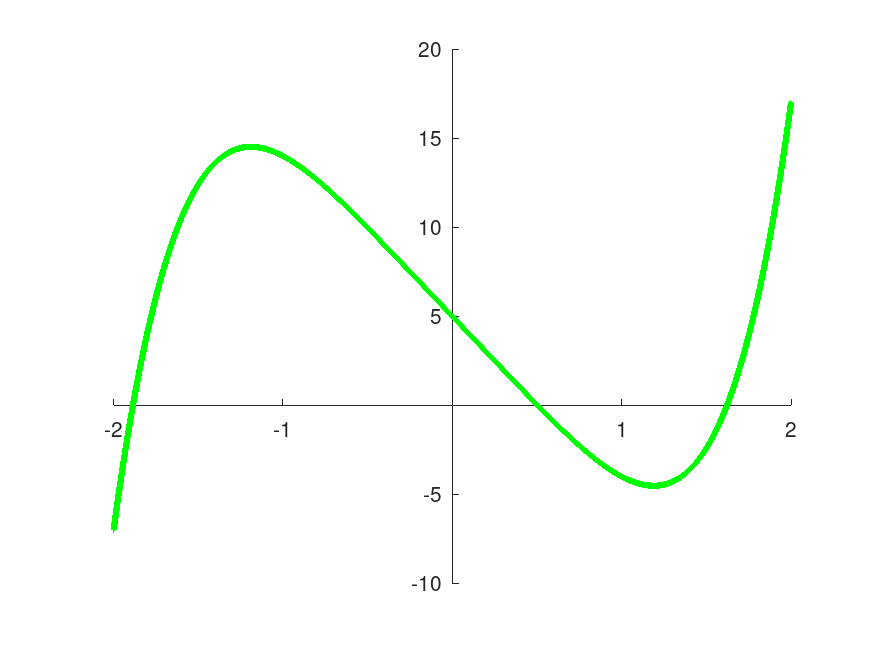
\includegraphics[width=10cm, height=3.2cm]{quantic2.png}
    \caption{\footnotesize Plotted by the ``GNU-Octave'', graph of \(f(x)=x^5-10x+5\) }
  \end{figure}
  The polynomial is \(f(x)=x^5-10x+5 \in \mathbb{Q}[x]\). Its graph is shown above.\\
 From its graph this polynomial has only three real roots. This polynomial is ``irreducible over \(\mathbb{Q}\) by the Eisenstein's criterion'' \cite{hunger} so by Theorem-11 its Galois group is \(S_5\) which contains \(5!=120\) elements.
 \end{example}

\begin{example}
  The polynomial is \(f(x)=x^7-2x^5-4x^3+2x^2+4x-2\) which is ``irreducible over \(\mathbb{Q}\) by the Eisenstein's criterion'' \cite{hunger}. Its graph is shown below.

    \begin{figure}[h!]
    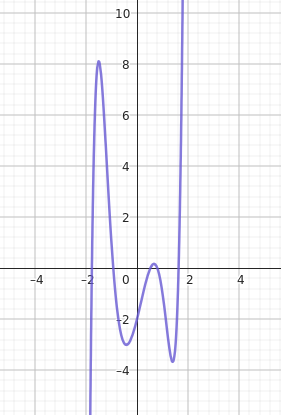
\includegraphics[width=10cm, height=5cm]{seventh2.png}
    \caption{\footnotesize Plotted by the ``Geogebra'', graph of \(f(x)=x^7-2x^5-4x^3+2x^2+4x-2\)}
  \end{figure}
The Graph shows this polynomial has exactly five real roots. So exactly two of its roots are complex. Hence by the Theorem-11 its Galois Group is \(S_7\) which contains \(7!=5040\) elements.
\end{example}

\subsection{Galois Group of Reducible polynomials}
For any polynomial \(f \in K[x]\) we factor \(f\) into irreducibles as \(f_1f_2...f_k\) and compute the Galois group \(G_i\)  of \(f_i\) for each \(i=1,2,...,k\). ``Then the Galois group \(G\) of \(f\) is isomorphic to a subgroup of \(\prod G_i\)'' \cite{algorithm}.

\begin{example}
  The polynomial is \(f(x) = x^4-7x^2+15\)\\
  Here, \(f(x)=(x^2-3)(x^2-5)\) so it is reducible over \(\mathbb{Q}\). Let \(f_1(x)=(x^2-3)\) and \(f_2(x)=(x^2-5)\). Then \(f_1,f_2\) are both irreducible over \(\mathbb{Q}\).\\

  The splitting field for \(f_1\) is \(\mathbb{Q}(\sqrt{3})\) so its ``Galois group is \({\mathbb{Z}}_2\)'' \cite{hunger}. The splitting field for \(f_2\) is \(\mathbb{Q}(\sqrt{5})\) so its Galois group is also \({\mathbb{Z}}_2\). Now we have the Galois group of \(f\) is a subgroup of \(G={\mathbb{Z}}_2 \times {\mathbb{Z}}_2\). \\

  Since the intersection of \(\mathbb{Q}(\sqrt{3})\) and \(\mathbb{Q}(\sqrt{5})\) is trivial the Galois group of \(f\) is \(G\) itself which is \textit{Klein 4-group}.
\end{example}

\begin{example}
  The polynomial is \(f(x)=x^7-5x^5-10x^3+5x^2+50x-25 \in \mathbb{Q}[x]\). This polynomial factors into irreducibles over \(\mathbb{Q}\) as \((x^2-5)(x^5-10x+5)\).\\
  The Galois group of \(x^2-5\) is \({\mathbb{Z}}_2\) \cite{algorithm} and of \(x^5-10x+5\) is \(S_5\) from the example-3. Also the roots of \(x^2-5\) are \(\sqrt{5}\) and \(-\sqrt{5}\) which are not the roots of \(x^5-10x+5\) from the its graph figure-4.1, so the intersection of the splitting fields of these two factor polynomials of \(f\) is trivial. Hence the Galois group of \(f\) is \(\mathbb{Z}_2 \times S_5\).
\end{example}

\subsection{Galois groups of Multi-variable Polynomials}
The Galois group of a polynomial in single variable can be generalized to the Galois group of a multi-variable polynomial.

\begin{example}
  The polynomial is \(f(x,y)=x+y \in \mathbb{Q}[x,y]\). Now the roots of \(f\) over all the complex numbers. Hence its Galois group is \(\mathbb{C}\).
\end{example}

\begin{example}
  The polynomials in \(\mathbb{Q}[x,y]\) are:
  \begin{align}
    y &= x^2+1 \\
    y &=x
  \end{align}
  The roots of these simultaneous polynomials are \(\omega, {\omega}^2\). Then the splitting field of this system is \(\mathbb{Q}(\omega)\). Here the automorphisms of \(\mathbb{Q}(\omega)\) are: \\
  \(\omega \longmapsto \omega\) and \hspace{9mm} \(\omega \longmapsto {\omega}^2\).\\
  Hence the Galois group of this system is \(\{(1), (12)\} \cong {\mathbb{Z}}_2\).
\end{example}

\subsection{The Classic Problem}
\begin{enumerate}
\item Is every polynomial equation solvable by the method of radicals?
\item Equivalently, does there exist an explicit "formula" which gives all solutions of a polynomial equation?
\end{enumerate}

If the degree of  the polynomial \(f\) is at most four then the answer is \textbf{yes} \cite{hunger}.\\

\textbf{Formulation of the Classic Problem}\\
The formula by the method of radicals means the formula involving only field operations and the extraction of \(nth\) roots \cite{hunger}.
The existence of a formula means there is a finite sequence of steps, each step being a field operation or the extraction of an \(nth\) roots, which yields all solutions of the given polynomial.
Performing a field operation leaves the base field unchanged, but the extraction of an \(nth\) root of an element
\(c\) in a field \(K\) amounts to constructing an extension field \(K(u)\) with \(u^n \in K\). Thus the existence of a formula for solving \(f(x)=0\) would imply
the existence of a finite tower of fields
\[K=E_0 \subset E_1 \subset ... \subset E_n\]
such that \(E_n\) contains a splitting field of \(f\) over \(K\) and for each \(i \geq 1\), \(E_i=E_{i-1}(u_i)\) with some positive power of \(u_i\) lying in \(E_{i-1}\) \cite{hunger}.\\
Conversely suppose there exists such a tower of fields and that \(E_n\) contains a splitting field of \(f\). Then
\[E_n = K(u_1,u_2,...,u_n)\]
and each solution is of the form \(f(u_1,...,u_n)/g(u_1,...,u_n)\) where \(f,g \in K[x_1,...,x_n]\). \\
Thus each solution is expressible in terms of a finite number of elements of \(K\), a finite number of field operations and \(u_1,...,u_n\). But
this amounts to saying that there is a formula for the solutions of the particular given equation \cite{hunger}. \\

\begin{definition} \cite{hunger} [Radical Extension]
  An extension field \(F\) of a field \(K\) is a radical extension of \(K\) if \(F=K(u_1,...,u_n)\), some power of \(u_1\) lies in \(K\) and for each \(i \geq 2\), some power of \(u_i\) lies in \(K(u_1,...,u_{i-1})\).\\
  The polynomial equation \(f(x)=0\) in rationals is \textit{solvable by radicals} if there exists a radical extension \(F\) of \(K\) and splitting field \(E\) of \(f\) over \(K\) such that \(F \supset E \supset K\).
\end{definition}

\begin{theorem} \cite{hunger}
If \(F\) is a radical extension of \(K\) and \(E\) is an intermediate field, then \(Aut_K^E\) is a solvable group.
\end{theorem}

\begin{corollary} \cite{hunger}
If the polynomial equation \(f(x)=0\) in rationals is solvable by radicals, then the Galois group of \(f\) is a solvable group.\\
\end{corollary}

\textbf{Group Theoretic Concepts}\\
\begin{definition} \cite{hunger} [Solvable Series]
  Let \(G\) be a group. A finite chain of subgroups \(G=G_0>G_1>...>G_n={e}\) such that \(G_{i+1}\) is normal in \(G_i\) for \(0 \leq i < n\) is called a subnormal series of \(G\). A subnormal series is a solvable series if each factor group \(G_i/G_{i+1}\) is abelian.
\end{definition}

\begin{definition} \cite{hunger} [Solvable Group]
A group is solvable if and only if it has a solvable series.
\end{definition}

If \(F\) is a radical extension of \(K\) then \(F\) is Galois over \(K\) and by the Fundamental Theorem of Galois \(Aut_K^E\) has a solvable series where \(E\) is an intermediate field. So \(Aut_K^E\) is solvable.

\subsubsection{Outcomes}
\begin{theorem} \cite{hunger}
The symmetric group \(S_n\) is not solvable for \(n \geq 5\).
\end{theorem}

The polynomial \(f(x)=x^5-10x+5 \in \mathbb{Q}[x]\) has Galois group ``\(S_5\), which is not a solvable group'' \cite{hunger}. The quintic polynomial equations over \(\mathbb{Q}\) are not solvable by radicals. That is there does not exist an explicit formula for solving the quintics. Moreover, ``polynomial equations of degree \(n \geq 5\) are not solvable by radicals'' \cite{hunger}.\\

\textbf{Illustrations}\\
Galois theory gives the precise condition under which a polynomial of degree \(n \geq 5\) is solvable by radicals or not.

\begin{example}
  The polynomial is \(x^5-1 \in \mathbb{Q}[x]\).\\
  The set of  roots of this polynomial are the fifth roots of unity which forms a group under addition modulo \(5\). Hence the ``Galois group is isomorphic to \(\mathbb{Z}_5\)'' \cite{hunger}. The group \(\mathbb{Z}_5\) is cyclic and ``every cyclic group is solvable'' \cite{galois}. Hence this polynomial is solvable by radicals.
\end{example}

\begin{definition} \cite{galois} [Cyclotomic Polynomial]
  The \(nth\)-cyclotomic polynomial is the polynomial \({\Phi}_n\) defined as \({\Phi}_n= \prod {(x-\zeta)}\), where \(\zeta\) is a primitive-\(nth\) of unity.
\end{definition}

\begin{theorem} \cite{galois}
  The Galois group of a \(nth\)-cyclotomic polynomial \({\Phi}_n\) of is \(\mathbb{Z}_n\).
\end{theorem}

\begin{example}
The polynomial is \(f(x)=x^{12}-x^{10}+x^8-x^6-x^2+1 \in \mathbb{Q}\)\\
which is a 58th-cyclotomic polynomial i.e this polynomial \(f(x)={\Phi}_{58}\).\\
  So its Galois group is \(\mathbb{Z}_{58}\), which is abelian and hence is solvable. Therefore this polynomial \(f(x)\) is solvable by radicals.
\end{example}

\vspace{9mm}
\section{Application to Coding Theory and Cryptography}
The loss of information is inevitable. It cannot be prevented or stopped. So, we need a way of retrieving the lost information or correcting the false information.

\begin{enumerate}
\item Paintings gets deteriorated over time and has to be renovated.
\item The data stored in a CD is lost over time \cite{coding}.
\end{enumerate}

To be able to detect and correct errors during transmission of information in digital system coding theory is developed. In digital system, information are transmitted as strings of \(0\) and \(1\). So the fundamental of the coding theory in computer system is the manipulation of strings of binary digits. The proper and complete manipulation of these strings is possibly only if the space of the strings is a field. This field is finite so this field is a Galois field. This is where the application of Galois theory comes. Another advantage of using field is that the space of code forms a vector space over the base field. \\
The widely used field for coding in electronically transmitting device is an extension field \({\mathbb{Z}}_2\) which is the field \(GF(2)\) consisting of \(0\) and \(1\). Recent works has shown that it is possible to extend codes to more general type of numbers called rings. This rings are called "Galois rings" \cite{error_correct}.\\

The non-empty set of symbols for the code \(\mathcal{A}\) called \textbf{alphabet}. A finite sequence of elements from \(\mathcal{A}\) is called a \textbf{word} over \(\mathcal{A}\). Let \(\mathcal{A}^*\) be the set of all words over \(\mathcal{A}\). A subset \(C\) of \(\mathcal{A}\) is called a code.
If the cardinality of the alphabet \(\mathcal{A}\) is \(q\) then the code \(C\) is called \(q-ary code\). For \(q=2\) it is called binary and for \(q=3\) it is called terniary \cite{error_correct}.

\subsection{Error-Correcting Codes}
The idea of coding theory is to append some extra digits to the information and use this to detect and possibly correct the errors during transmission.
\begin{definition} \cite{coding} [Error-Correcting Codes]
  These codes that can correct themselves are called Error correcting codes.
\end{definition}

\textbf{Linear Codes}
Let \(K=GF(q)\) be a Galois field. Then a finite extension of \(K\) of dimension \(n\) is \(V=GF(q)^n=GF(q^n)\).\\[3mm]
A linear code \(C\) is a subspace of \(V\). The code \(C\) has dimension \(k \leq n\) and the length \(n\). It is called a ``\((n,k)\) code'' \cite{error_correct}.\\[5mm]


The usefulness of linear code is that they are vector spaces over the base field so they have a basis. All the code words can be generated with this basis. Instead of storing all \(2^k\) number of code words (for \(k\)-dimensional binary codes), storing only \(k\) basis elements is sufficient which saves massive storage.\\[2mm]
Let \(C\) be \((n,k)\) code which is a subspace of \(V\).
\vspace{5mm}

\begin{definition} \cite{error_correct} [Generator Matrix]
  Let \(\{v_1, v_2,...,v_k\}\) be a basis of \(C\). A generator matrix is the \(k \times n\) matrix \(G=\begin{pmatrix} \small
      v_1\\
      v_2\\
      ...\\
      v_k
    \end{pmatrix}
  \).
\end{definition}

\vspace{5mm}

\begin{definition} \cite{error_correct} [Parity check matrix]
  ``The dual code of \(C\) is the set \(C^{\perp}=\{x \in V \;| \; x.y=0 \;\; \forall y \in V \}\) \cite{error_correct}. The dual code is a code in itself and has dimension \(n-k\).\\
  The \(C^{\perp}\) is linear so it has a generator matrix.A generator matrix \(H\) of \(C^{\perp}\) is called a parity check matrix.
\end{definition}
\vspace{5mm}

\begin{theorem} \cite{coding}
  If \(G=(I_{k \times k},A_{k \times (n-k)})\) is a generator matrix of an \((n,k)\) code \(C\) then its parity check matrix is \(H=(I_{(n-k) \times (n-k)}, A'\) where \(A'\) is the transpose of \(A\).
\end{theorem}
\vspace{5mm}

\begin{definition} \cite{error_correct}
  The \textit{Hamming distance} between \(v,w \in V\) is defined by \(d_h(v,w)=|\{i\;|\; v_i \neq w_i;\; 1 \leq i \leq n \}|\).\\
  The \textit{minimum distance} of a code \(C\) is defined as \(min\{d_h(v,w)\;|\; d_h(v,w) \neq 0, v,w \in C\}\).\\
  The weight of a vector is its distance from zero and the \textit{minimum weight} of a code \(C\) is the minimum weight of all non-zero weights of the vectors in \(C\).
\end{definition}

\begin{theorem} \cite{error_correct}
  A linear code \(C\) with minimum weight \(d\) can correct strings having number of errors up to \(t= \lfloor (d-1)/2 \rfloor\).\\
\end{theorem}
\clearpage

\textbf{Syndrome Correcting}\\
\begin{definition}
  The syndrome of a vector \(y \in V\) is defined as \\ \(syn(y)=\begin{pmatrix} \small
    y.h_1\\
    y.h_2\\
    ...\\
    y.h_{n-k}
  \end{pmatrix}\), \hspace{12mm} where \(\begin{pmatrix}
    h_1 \\ h_2\\ ...\\ h_{n-k}
  \end{pmatrix}\) is the parity check matrix of \(C\) \cite{error_correct}.
\end{definition}
Now the code \(C\) is a subgroup of \(V\) under addition. Moreover, it is a normal subgroup of \(V\).

\begin{theorem} \cite{error_correct}
  Two vectors in \(V\) have the same syndrome if and only if they are in the same co-set of \(C\).
\end{theorem}

\textbf{Illustration}\\
To apply \((n,k)\) coding first we need to group our information into blocks of length \(k\).
\(u_1,...,u_k\),  \(u_k,...,u_{2k}\),... . This space has dimension \(k\). Now these block of codes are encoded separately each to a code of length \(n\) as shown \cite{coding}.

\begin{tikzpicture}
  \hspace{1cm}
  \node [] (u) {\((u_1,u_2,...,u_k\))};
  \node[
  right of=u,
  rectangle,
  draw,
  thick,
  fill=gray!10,
  minimum width=30mm,
  minimum height=13mm,
  xshift=35mm] (e) {\bfseries Encoder};

  \node[right of=e, xshift=35mm] (x) {\((x_1,x_2,...,x_n)\)};

  \draw[->,ultra thick] (u)--(e);
  \draw[->,ultra thick] (e)--(x);
\end{tikzpicture}

\noindent
Mathematically, the encoded vector \(x\) is obtained form the original vector \(u\) using the generator matrix \(G\) by the relation \(x=uG\) \cite{coding}.\\[5mm] To continue and complete the diagram.\\

\begin{tikzpicture}
  \hspace{-5mm}
  \node[
  rectangle,
  draw,
  thick,
  fill=gray!20,
  minimum width=13mm,
  minimum height=8mm,
  ] (t) {Transmission};

  \node[below of=t, yshift=-9mm] (y) {\small \((y_1,y_2,...,y_n\))};

  \node[
  left of=y,
  rectangle,
  draw,
  thick,
  fill=gray!20,
  minimum width=13mm,
  minimum height=8mm,
  xshift=-20mm] (c) {Corrector};

  \node[left of=c, xshift=-20mm] (x) {\small \((x_1,x_2,...,x_n)\)};

  \node[
  left of=x,
  rectangle,
  draw,
  thick,
  fill=gray!20,
  minimum width=13mm,
  minimum height=8mm,
  xshift=-20mm] (d) {Decoder};

  \node[left of=d, xshift=-20mm] (u) {\small \((u_1,u_2,...,u_k\))};


  \draw[->,very thick] (0,1)--(t);
  \draw[->,very thick] (t)--(y);
  \draw[->,very thick] (y)--(c);
  \draw[->,very thick] (c)--(x);
  \draw[->,very thick] (x)--(d);
  \draw[->,very thick] (d)--(u);
\end{tikzpicture}

\vspace{4mm}

\textbf{Correcting Process}\\
Suppose the signal received is the vector \(y\).
\begin{enumerate}
\item First we determine its syndrome, \(syn(y)\).
\item Determine the co-set of \(C\) containing \(syn(y)\), say \(e + C\).
\item Then \(y=e+x\) for some \(x \in C\). This implies \(x=y-e\). Since \(x \in C\), this \(x\) is the required correction of \(y\) \cite{error_correct}.
\end{enumerate}
This \(e\) is also called "error vector" \cite{error_correct}.

\begin{example}
  Consider a generator matrix \( \small G=\begin{pmatrix}
    1 & 0 & 1 & 0\\
    0 & 1 & 1 & 1
  \end{pmatrix}\). Then the parity check matrix is \(H=\begin{pmatrix}
    1 & 1 & 1 & 0\\
    0 & 1 & 0 & 1
  \end{pmatrix}\). And the code generated by \(G\) is \\ \(C=\{(0,0,0,0),(1,0,1,0),(0,1,1,1),(1,0,1,1)\} \;\; \subset GF(2^{4})\).\\

  Suppose the received vector is \(y=(1,1,1,0)\). Then \(y \not \in C\) so the information is distorted from the original information. To get the original information:\\
  \(syn(y)= \begin{pmatrix}
    y.h_1 \\ y.h_2
  \end{pmatrix} = \begin{pmatrix}
    1 \\ 1
  \end{pmatrix}\) where \(h_1\) is the first row and \(h_2\) is the second row of \(H\).\\
  Now if \(e=(0,1,0,0)\) then \(e+C=\begin{pmatrix}
    1 \\ 1
  \end{pmatrix}\) so \(y-e=(1,1,1,0)-(0,1,0,0)=(1,0,1,0) \in C\) is the original information \cite{error_correct}.
\end{example}

\subsubsection{Perfect Code}
The code \(C \subseteq V\) as of above is perfect if the union of all the spheres of radius \(t\) about its code-words is the vector space \(V\).\\
This code is \(C\) is called perfect because every received vector with the number of errors given by \(t\) can be corrected to a code-word of \(C\) \cite{error_correct}.

\begin{example}
  The code \(C=V\) is a perfect code. This code cannot correct any errors because every possible code word is in the \(C\). Therefore this perfect code is trivial \cite{error_correct}.
\end{example}

\begin{example}
  The general binary Hamming code \(H_r\), \(r \in \mathbb{N}\) whose parity check matrix \(H\) column consisting of non-zero r-tuples \cite{error_correct}.
\end{example}

\subsubsection{Cyclic Code}
The code \(C\) as of above is cyclic if \((a_0,a_1,...,a_{n-1}) \in C\\ \implies (a_{n-1},a_0,...,a_{n-2}) \in C\).\\
Suppose \(C\) is a code over a Galois field \(F=GF(q)\). Then there exist a correspondence \(\Phi : C \mapsto F[x]/(x^n-1)\) such that \(\{(a_0,a_1,...,a_{n-1}),(a_1,...,a_{n-1},a_0),....,(a_{n-1},a_0,....,a_{n-2})\} \longmapsto a_0+a_1x+a_2x^2+...+a_{n-1}x^{n-1}\). This map \(\Phi\) is homomorphism.This shows that the cyclic code \(C\) can be embedded into the ring \(R_n=F[x]/(x^n-1)\) \cite{error_correct}.

\begin{theorem} \cite{error_correct}
  \begin{enumerate}
  \item A subset \(S\) of \(R_n\) corresponds to a cyclic code if and only if \(S\) is an ideal of \(R_n\) and
  \item if \(S=(g(x))\) if and only if  \(g(x)\) divides \(x^n-1\).
  \end{enumerate}
\end{theorem}

 This theorem determines all cyclic codes. They are ideals of \(R_n\) and these ideals are generated by the polynomials that divides \(x^n-1\). Thus cyclic code have a generator polynomial which is computationally simpler than having a generator matrix. \\[2mm]
  This is where usages of polynomial representation of finite fields come into play and this is where cyclic code has advantage over general linear code.

\begin{example}
  The divisors of \(x^3-1 \in F=GF(2^{3})\) are \(1, x+1, x^2+x+1, x^3-1\).\\
  For \(g(x)=x+1\) we have \(F[x]/(g(x))=\{(0),(1+x),(1+x^2),(x+x^2)\}\) so the corresponding cyclic code is \(\{(0,0,0),(1,1,0),(1,0,1),(0,1,1)\}\) \cite{error_correct}.
\end{example}

\textbf{Usages}\\
\begin{enumerate}
\item The \((3,1)\) binary code is used in the short-range wireless communication system like \(Bluetooth^{TM}\) \cite{wireless}.
\item The Hamming Code \((7,4)\) is used in memory devices like RAM \cite{coding}.

\item The Cyclic codes are used in storing data in CDs and DVDs \cite{coding}.
\end{enumerate}


\subsection{Cryptography}
\noindent It is the science of safe-guarding information by converting the original message into something unreadable. Galois Fields are the life of modern cryptography used in digital communication.\\

\textbf{Advance Encryption Standard(AES)}\\
The Advance Encryption Standard is a Computer Security Standard for cryptography which is approved by the ``Federal Information Processing Standards Publications'' of USA which became effective on May 26, 2002. ``The AES algorithm is a \textit{symmetric block cipher} that can encrypt and decrypt digital information'' \cite{aes}. Symmetric key cryptography is used to share information between two parties where the two parties share a secret ``key'' and a public encryption algorithm \cite{wireless}. The generic algorithm of AES consists of smaller sub-algorithms namely ``Sub-Bytes, Shift-Rows, Mix-Columns and Add-Round-Key'' \cite{aes}.


\subsubsection{The State}
First the data is broken into blocks and each block is broken into smaller chunks of a size byte (16 bytes for a block of size 128bits). This block is then represented in a  which consisting of bytes of the word. This matrix is called the State.\\
Mathematical operations are not applicable to the data directly so the significance of this step is to make the data applicable for mathematical operations.\\
For the 128-bit key encryption the algorithm forms a \(4 \times 4\) matrix with each entry of a size one byte. This matrix can afford to evaluate a data of size 16 byte at a time \cite{aes}.

\subsubsection{Sub-Bytes}
In this step, first each byte of the matrix is replaced with its multiplicative inverse if it has one. Then it transforms each bytes using an invertible affine transformation, \(x \mapsto Ax+b\) \cite{aes}.

\subsubsection{Mathematical Preliminaries}
Each byte in the state i.e each entry in the matrix, is interpreted as one of the 256 elements of a finite field \(GF(2^8)\). Then the addition, multiplication operations are performed according to the respective field operations of the field \(GF(2^8)\).

\subsubsection{Shift-Rows}
In this step entries of a row is shifted to scramble data. Row-n shifted to the left by \(n-1\) unit. Here,\\
\(1-1=0\), so row-1 is left unchanged. \(2-1=1\), so row-2 is shifted to the left by 1 unit and row-3 by 2 unit and so on as shown below \cite{aes}.

If \(A=\begin{bmatrix}
    a_{11}&a_{12}&a_{13}&a_{14}\\
    a_{21}&a_{22}&a_{23}&a_{24}\\
    a_{31}&a_{32}&a_{33}&a_{34}\\
    a_{41}&a_{42}&a_{43}&a_{44}
    \end{bmatrix}\) \hspace{3mm} then \(A'=\begin{bmatrix}
    a_{11}&a_{12}&a_{13}&a_{14}\\
    a_{22}&a_{23}&a_{24}&a_{21}\\
    a_{33}&a_{34}&a_{31}&a_{32}\\
    a_{44}&a_{41}&a_{42}&a_{43}
    \end{bmatrix}\)  is the matrix after Shit-Row.

\subsubsection{Mix-Columns}
In this step each column is transformed using a linear transformation, \(c \mapsto Bc\) where \(c\) is a column of the matrix obtained above. Since linear transformation is invertible this step is invertible. Note every step of this algorithm must be invertible to be able to decrypt the data \cite{aes}.

\subsubsection{Add-Round-Key}
This is the step where the encrypted data gets uniqueness. Each user is assigned an "unique key" and this key is added to the matrix obtained from the last step \cite{aes}.\\[7mm]


\textbf{Illustration}\\
Let us encrypt the sentence "Fun Cryptography". This consists of exactly 16 characters.
\begin{enumerate}
\item First we write the ASCII representation of each character of the sentence as shown below. We do so because the ASCII representation gives the binary representation of each character which has a size of a byte. The ASCII representation of "F" is \(70\) which is \(01000110\) in binary.
  \[\begin{bmatrix}
      70 & 117 & 110 & 32 \\
      67 & 114 & 121 & 112\\
      116 & 111 & 103 & 114 \\
      97 & 112 & 104 & 121
    \end{bmatrix}=
    \begin{bmatrix}
      01000110 & 01110110 & 01101110 & 00010000 \\
      01000011 & 01110010 & 01111001 & 01110000\\
      01110100 & 01101111 & 01100111 & 01110010 \\
      01100001 & 01110000 & 01101000 & 01111001
    \end{bmatrix}
  \]


\item After performing Sub-Bytes, Shift-Rows, Mix-Columns, we get the following matrix.

  \[\begin{bmatrix}
      11100111 & 00011000 & 00100100 & 01110000\\
      00101010 & 10101011 & 00111001 & 01100011\\
      00010101 & 01100101 & 11110111 & 10100111\\
      10101011 & 11110110 & 00000011 & 10100100
    \end{bmatrix}=
    \begin{bmatrix}
      231 & 24 & 36 & 112\\
      42 & 171 & 57 & 99\\
      21 & 101 & 247 & 167\\
      171 & 246 & 3 & 164
    \end{bmatrix}
  \]

\item We have omitted the Add-Round-Key step just for the sake of simplicity. The matrix obtained at last in step-2 translates to something different from our original sentence.

\item The decryption process is applying the inverse of the encryption process \cite{aes}.
\end{enumerate}
\clearpage

%-------------------------------------------------------------------------------------------
\textbf{Conclusions}\\
The Galois theory that begun in the 19th century due to the french mathematician \textit{Évariste Galois} is still a relevant field of research today. Over the 200 years this theory has found its development as a linking theory of the two main theories: Group Theory and Field theory. It has found its applications in both pure and applied mathematics; where-ever ``Field Theory'' has anything to do with.\\
Many concepts of Abstract algebra, Algebraic number theory, Algebraic geometry, etc rely heavily on Galois theory because they are developed on field extensions, and the computer science relies heavily on Galois field.\\


\vspace{3mm}
\textbf{Acknowledgment:} \\
I would like to thank \textit{Kathmandu Center for Research and Education Chinese Academy of Sciences-TU} for awarding me with \\
\textit{KCRE Excellent Student Thesis Grant 2023(Grant number: 08092023).}
\vspace{7mm}

%-----------------------------------------------------------------------------------------------------------------
\begin{thebibliography}{9}
\bibitem{galois}
Escofier, J. P. (2000) \emph{Galois Theory}. Springer, New York.

\bibitem{error_correct}
Holdman, G. R. (2019) \emph{Error Correcting Codes  Over Galois Rings}. Graduate Dissertation, Department of Mathematics, Whitman college, 345 Boyer Ave.
Walla Walla, Washington, U.S.A.

\bibitem{hunger}
Hungerford, T. W. (2012) \emph{Algebra}. Springer (India), New Dheli.

\bibitem{algorithm}
Lenstra, A., Lenstra, H.,  \& Lovasz, L. (1982)  Factoring polynomials with rational coefficients. \emph{Mathematische Annalen},261,12.

\bibitem{coding}
Neubaer, A.,  Freudenberger, J.,  \& Kuhn, V. (2007) \emph{Coding Theory, Algorithms, Architectures, and Applications}. John Wiley and Sons Ltd, Chichester, West Sussex, England:1-93.

\bibitem{wireless}
Sarma, D. (2018) Implementation of Galois Field for Application in Wireless Communication Channels. \emph{MATEC Web of Conferences},2010:03012.

\bibitem{aes}
National Institute of Standards and Technology. (2001) Advanced Encryption
Standard (AES). \emph{(Department of Commerce, Washington, D.C.), Federal Information Processing Standards Publication (FIPS) NIST FIPS}. 197-upd.1 updated May 9, 2023. doi:10.6028/NIST.FIPS.197-upd1.
\end{thebibliography}

\end{document}



%%% Local Variables:
%%% mode: latex
%%% TeX-master: t
%%% End:
